%%
% 引言或背景
% 引言是论文正文的开端,应包括毕业论文选题的背景、目的和意义;对国内外研究现状和相关领域中已有的研究成果的简要评述;介绍本项研究工作研究设想、研究方法或实验设计、理论依据或实验基础;涉及范围和预期结果等。要求言简意赅,注意不要与摘要雷同或成为摘要的注解。
% modifier: 黄俊杰(huangjj27, 349373001dc@gmail.com)
% update date: 2017-04-15
%%
\usetikzlibrary{shapes,arrows,positioning}

\chapter{绪论}
%定义,过去的研究和现在的研究,意义,与图像分割的不同,going deeper
\label{cha:introduction}
\section{研究背景}
\label{sec:background}
% What is the problem
% why is it interesting and important
% Why is it hards, why do naive approaches fails
% why hasn't it been solved before
% what are the key components of my approach and results, also include any specific limitations,do not repeat the abstract
%contribution
在航空航天、能源动力及环境工程等领域,流场特性分析是气动设计、设备优化及流动控制的核心基础。以无人机气动外形设计为例,翼型表面压力分布、边界层分离特性及尾流涡结构的精确获取,直接影响无人机的升力效率、阻力特性及抗结冰性能。然而,传统计算流体力学(CFD)方法依赖精细化网格划分与长时间数值迭代,对 NACA0012 等典型翼型进行全工况模拟时,单工况计算耗时可达数小时至数天,难以满足工程设计中多参数快速迭代的需求。尤其在无人机防除冰设计中,需实时评估不同结冰厚度、液态水含量对翼型流场的影响,传统 CFD 方法的高计算成本成为技术瓶颈。
本征正交分解(proper orthogonal decomposition,POD)方法由 Lumley\textsuperscript{\cite{lumley1967structure}} 提出,其思想为将流场分解为若干正交的空间模态,依据模态能量大小进行排序,通过线性叠加前几阶高阶模态实现原流场的精确重构。因 POD 方法可对流场实现
时空解耦,在低速圆柱绕流\textsuperscript{\cite{wang2023}}、翼型流动\textsuperscript{\cite{sun2022analysis}} 等领域得到了推广应用。近年来,POD 方法发展为可从一系列流场“快照”矩阵中提取出本征模态,并通过模态能量占比排序采用部分模态表征流场绝大部分特征,实现原始流场的重构,已被广泛应用在非定常流场数据处理以及流动特征性分析等方面。在航空、能源等领域,流场参数的精确预测对飞行器设计、能源设备优化至关重要。\textsuperscript{\cite{HKDI202407028}}
NACA0012 翼型作为对称翼型的经典代表,其流场特性随攻角变化呈现丰富的流动现象:小攻角时为附着流动,中等攻角时出现边界层分离,大攻角时形成显著分离涡,是研究流动分离、失速特性的理想对象。然而,该翼型在跨音速流动时的激波 - 边界层干扰、结冰条件下的外形畸变对流场的影响,均需高效的流场重构方法支撑。目前,工程中仍依赖全尺寸 CFD 模拟获取流场数据,缺乏适用于多工况快速预测的高效工具。因此,构建基于 POD 的 NACA0012 翼型流场重构方法,对提升无人机气动设计效率、降低研发成本具有重要现实意义。



%%引言是论文正文的开端,应包括毕业论文选题的背景、目的和意义;对国内外研究现状和相关领域中已有的研究成果的简要评述;介绍本项研究工作研究设想、研究方法或实验设计、理论依据或实验基础;涉及范围和预期结果等。要求言简意赅,注意不要与摘要雷同或成为摘要的注解。
\section{研究目的和意义}
本研究致力于深入探究基于 POD 降阶模型的流场重构方法,重点聚焦于插值 POD 方法在翼型流场分析中的应用。研究旨在实现两大核心目标:一是显著提升流场重构的精度,使重构后的流场能够高度还原真实流场的复杂特性,包括压力分布、速度梯度以及涡量等关键物理量的准确再现\cite{Smith2020};二是大幅提高流场重构的效率,降低计算成本,缩短计算时间,满足实际工程中对快速、准确流场分析的迫切需求\cite{Jones2019}。

具体而言,本研究选取经典的 NACA0012 翼型模型作为研究对象,运用插值 POD 方法对其流场进行精确重构\cite{Lee2021}。通过与专业 CFD 软件模拟生成的真实数据进行全面、细致的对比分析,系统验证插值 POD 方法在流场重构中的有效性和准确性\cite{Wang2022}。这一研究过程不仅有助于深入理解 POD 降阶模型在流场重构中的内在作用机制,揭示其背后的数学原理和物理意义\cite{Cao2020},还能为实际工程应用提供可靠、实用的技术手段。

在实际工程应用中,准确的流场重构结果能够为翼型的优化设计提供坚实的科学依据。工程师可以根据重构后的流场信息,有针对性地调整翼型的几何参数,如翼型厚度、弯度以及前缘半径等,设计出更高效、更节能的翼型\cite{Yang2023}。例如,通过流场重构发现翼型前缘的压力集中问题,可以优化前缘形状,降低压力峰值,减少阻力,提高升阻比\cite{Zhang2018}。同时,本研究成果还可以为风力发电叶片设计\cite{Chen2021}、船舶水动力性能优化\cite{Liu2022}等相关领域提供有益的借鉴和参考,推动整个相关领域的技术创新和发展,为社会经济的可持续发展做出贡献。
\section{国内外研究现状和相关工作}
\label{sec:related_work}
\subsection{ POD 降阶模型的研究现状}
POD 方法最早由 Kosambi 于1943年提出\cite{Kosambi1943},经过多年的发展,在理论研究和实际应用方面均取得了长足进步。在理论层面,众多学者致力于改进 POD 模型,以增强其对复杂流场的适应性和重构精度。例如,为了更好地捕捉流场中的动态变化特性,研究者引入时间延迟嵌入技术\cite{Schmid2011},将时间序列中的历史信息融入 POD 分析中。通过构建时间延迟坐标系统,POD 模型能够有效提取流场中的动态特征,如涡旋的生成、演化和消散过程\cite{Rowley2009}。多尺度分析方法的引入也是理论研究的重要进展之一。该方法通过将流场分解为不同尺度的成分,分别进行 POD 分析,能够更细致地描述多尺度复杂流场的特性\cite{Lumley2017}。例如,在研究大气边界层流场时,多尺度 POD 分析可以清晰地分离出大尺度的湍流结构和小尺度的粘性耗散区域\cite{Taira2020},为深入理解大气边界层的物理过程提供了有力工具。

在应用领域,POD 模型凭借其高效性和准确性,已广泛应用于多个学科。
 航空航天领域:POD 模型被用于飞行器气动性能的优化设计\cite{LeGresley2006}。通过对飞行器周围流场的降阶重构,工程师可以快速评估不同设计方案的气动性能,如升力系数、阻力系数以及力矩系数等,从而加速飞行器的设计优化进程。
 
 汽车工业:POD 模型被用于汽车外流场的模拟和优化\cite{Bergmann2018},通过降低计算成本,缩短新车研发周期。
 
 能源领域:POD 模型被应用于风力发电机叶片的气动性能分析和优化\cite{Couplet2003},提高风能转换效率。
 
 尽管 POD 模型取得了显著进展,但目前的研究仍存在一些局限性。在面对高度非线性的流场时,POD 模型的重构精度有待进一步提高\cite{Holmes2012}。非线性流场中存在的复杂物理现象,如混沌行为、分岔现象等,给 POD 模型的准确描述带来了挑战\cite{Noack2003}。此外,在一些对实时(2025年05月04日)性要求极高的应用场景,如飞行器的实时(2025年05月04日)飞行控制、工业过程的在线监测与优化等,POD 模型的计算速度仍需进一步优化\cite{Peherstorfer2021}。传统的 POD 计算方法在处理大规模数据时,计算时间较长,难以满足实时(2025年05月04日)性需求。因此,如何提高 POD 模型在非线性流场中的重构精度和计算速度,是当前研究的重点和难点问题\cite{Carlberg2023}。

%%ljx论文
\subsection{流场重构方法的研究现状}
目前,流场重构方法主要分为传统方法和基于机器学习的方法两大类。
传统流场重构方法包括插值法、有限元法等。插值法在处理简单流场时具有较高的精度和计算效率\cite{Press2007}。例如,在已知有限个离散点的流场数据时,通过线性插值或样条插值等方法,可以快速估算流场中其他位置的物理量值\cite{Boyd2001}。有限元法则是将计算区域离散化为有限个单元,通过求解每个单元上的控制方程来重构流场\cite{Zienkiewicz2013}。在处理规则几何形状的流场时,有限元法能够提供较为准确的结果\cite{Bathe2014}。然而,当面对复杂流场时,传统方法的局限性逐渐凸显。复杂流场中的不规则边界、多尺度流动结构以及强非线性特性,使得传统方法需要大量的计算资源和时间,且难以处理大规模的数据\cite{Taylor2013}。例如,在模拟具有复杂地形的大气边界层流场时,传统方法需要生成极其细密的网格来捕捉地形细节,导致计算量呈指数级增长,且计算精度仍难以保证\cite{Moin2012}。

基于机器学习的流场重构方法近年来成为研究热点。深度学习中的卷积神经网络(CNN)和循环神经网络(RNN)在流场数据的特征提取和重构方面展现出强大的能力\cite{Goodfellow2016}。CNN 能够通过卷积层和池化层自动提取流场数据中的空间特征,对复杂的流场结构具有良好的识别能力\cite{Krizhevsky2012}。RNN 则可以处理流场数据中的时间序列信息,适用于动态流场的重构\cite{Hochreiter1997}。将 CNN 和 RNN 相结合的方法,如长短期记忆网络(LSTM),在流场重构中取得了较好的效果\cite{Graves2013}。然而,这些基于机器学习的方法也存在一些问题。首先,它们对数据量的需求巨大,需要大量的高质量训练数据来保证模型的准确性\cite{LeCun2015}。获取和标注这些数据往往需要耗费大量的时间和资源\cite{Sun2021}。其次,机器学习方法对计算资源的要求极高,需要高性能的图形处理单元(GPU)集群来支持模型的训练和运行\cite{Schmidhuber2015}。此外,机器学习模型的可解释性较差,难以直观地理解模型的决策过程和结果\cite{Rudin2019},这在一些对可靠性和安全性要求较高的工程应用中是一个重要的限制因素\cite{Arrieta2020}。

相比之下,基于 POD 降阶模型的流场重构方法在计算效率和模型可解释性方面具有明显优势。POD 降阶模型通过数学变换提取流场的主要特征,计算过程相对简单,计算效率高\cite{Berkooz1993}。同时,POD 模型的基函数具有明确的物理意义,能够直观地反映流场的主要结构,使得模型的结果具有较好的可解释性\cite{Holmes2012}。例如,POD 基函数可以对应流场中的大尺度涡旋结构或平均流场特征\cite{Lumley2017},便于工程师理解和分析。因此,基于 POD 降阶模型的流场重构方法受到了越来越多的关注,成为当前流场重构领域的研究重点之一\cite{Taira2020}。然而,如何进一步提高其在复杂流场中的重构精度,以及如何与机器学习等新兴技术相结合\cite{Carlberg2023},仍然是有待深入研究的课题。
%%基于目标压力分布优化的翼型反设计方法研究_李焦赞
\section{研究内容与方法}
\subsection{研究内容}
本研究涵盖多个关键方面。首先,深入剖析 POD 降阶模型的基本理论,包括基本 POD 方法和 Snapshot POD 方法的详细原理及严谨的数学推导。基本 POD 方法通过寻找一组最优的正交基函数,将高维流场数据投影到低维空间,实现数据的高效降维与准确重构。在数学推导过程中,基于泛函分析和线性代数理论,详细阐述如何通过求解特征值问题得到 POD 基函数。Snapshot POD 方法则针对基本 POD 方法计算量过大的问题,通过对采样数据的巧妙处理,大幅降低计算复杂度。具体而言,Snapshot POD 方法利用采样数据构建低阶自相关矩阵,从而简化特征值求解过程,提高计算效率。
其次,构建精确的 NACA0012 翼型模型,并运用专业 CFD 软件模拟生成该翼型在不同工况下的压力数据。在建模过程中,严格遵循 NACA0012 翼型的标准几何参数,确保模型的准确性。模拟工况涵盖不同的迎角(从 0° 到 3°,以 0.2° 为间隔)、马赫数(从 0.7 到 0.8,以 0.005 为间隔))等参数组合,以真实模拟翼型在实际飞行中的各种复杂情况。

然后,详细研究插值 POD 方法在流场重构中的具体应用,包括该方法的算法原理和具体实现步骤。插值 POD 方法通过对采样解的深入分析,建立扰动变量与基系数之间的连续函数关系。具体采用三次样条插值等方法,实现对非采样工况下流场的准确预测。在算法实现过程中,详细阐述如何确定插值节点、构建插值函数以及求解基系数等关键步骤。

最后,将插值 POD 方法预测的数据与 CFD 软件模拟生成的真实数据进行全面对比,展开深入的数据分析。对比不同工况下的压力分布,从重构精度、计算效率等多个维度评估插值 POD 方法在流场重构中的性能。在重构精度评估方面,采用均方根误差(RMSE)、平均绝对误差(MAE)等指标定量分析预测数据与真实数据的偏差。在计算效率评估方面,对比插值 POD 方法与传统 CFD 方法的计算时间,分析其在不同工况下的加速比。

\subsection{研究方法}
本研究采用理论研究与数值模拟紧密结合的方法。在理论研究方面,系统学习 POD 降阶模型和插值 POD 方法的相关理论知识。深入研读国内外权威文献,全面掌握 POD 方法的数学基础,包括泛函分析中的内积空间理论、线性代数中的特征值与特征向量计算等知识,深刻理解其在流场重构中的应用原理。同时,对插值 POD 方法的算法设计、误差分析等方面进行深入研究,为后续的数值模拟提供坚实的理论支撑。例如,在误差分析中,通过理论推导建立插值误差与采样点数量、流场复杂度之间的定量关系,为优化插值 POD 算法提供理论依据。

在数值模拟方面,选用专业 CFD 软件,如 ANSYS Fluent、OpenFOAM 等,对 NACA0012 翼型模型进行精确建模。在建模过程中,依据翼型的几何参数,利用软件的几何建模功能创建精确的翼型形状。设置模拟的边界条件时,物面边界采用绝热的无滑移边界条件,以准确模拟气流与翼型表面的实际相互作用;远场边界采用无反射边界条件,有效减少边界对内部流场的干扰。选择合适的湍流模型,如 k - ω 湍流模型,以精确模拟翼型周围的湍流流动。在空间离散方面,采用格心格式的有限体积法,将计算区域划分为大量的网格单元,通过对每个单元内的守恒方程进行离散求解,得到流场的数值解。在时间推进方面,运用显式 5 步龙格库塔迭代方法,逐步求解流场随时间的变化。同时,对网格的划分进行精细化处理,通过网格无关性验证,确定最优的网格密度,确保模拟结果的准确性和可靠性。

利用模拟生成的数据,运用插值 POD 方法进行流场重构。通过编写相应的计算程序,实现插值 POD 方法的各个计算步骤,包括 POD 基的计算、基系数的求解以及插值计算等。在程序编写过程中,采用高效的算法和数据结构,提高计算效率。最后,通过对比分析插值 POD 方法预测的数据与真实数据,验证该方法的有效性和准确性。在对比分析过程中,运用可视化技术,如等值线图、矢量图等,直观展示预测结果与真实结果的差异,为进一步优化插值 POD 方法提供直观依据。
\subsection{技术路线}
研究遵循 “数据生成 - 特征提取 - 模型构建 - 实验验证” 的技术路线(图 1.1):首先通过 CFD 软件获取多攻角、多马赫数流场数据,经标准化处理后进行 POD 分解,筛选累计能量占比达 95\%以上的主导模态;继而采用三次样条插值建立攻角、马赫数等参数与模态系数的映射关系,构建流场重构模型;最后通过压力系数分布对比,验证模型在典型工况下的重构精度,并分析模态截断误差与插值误差的影响规律。
\begin{figure}[h]
    \centering
    \begin{tikzpicture}[node distance=2cm]

        % 定义样式
        \tikzstyle{startend} = [rectangle, rounded corners, minimum width=3cm, minimum height=1cm, text centered, draw=black, fill=red!30]
        \tikzstyle{process} = [rectangle, minimum width=3cm, minimum height=1cm, text centered, draw=black, fill=orange!30]
        \tikzstyle{decision} = [diamond, minimum width=3cm, minimum height=1cm, text centered, draw=black, fill=green!30]
        \tikzstyle{arrow} = [thick,->,>=stealth]

        % 创建节点
        \node (start) [startend] {开始};
        \node (data) [process, below of=start] {CFD软件获取多攻角流场数据};
        \node (preprocess) [process, below of=data] {数据标准化处理};
        \node (pod) [process, below of=preprocess] {POD分解};
        \node (mode) [process, below of=pod] {筛选主导模态(累计能量占比>95\%)};
        \node (interpolation) [process, below of=mode] {三次样条插值建立映射关系};
        \node (model) [process, below of=interpolation] {构建流场重构模型};
        \node (validation) [process, below of=model] {多工况对比实验验证};
        \node (end) [startend, below of=validation] {结束};

        % 连接节点
        \draw [arrow] (start) -- (data);
        \draw [arrow] (data) -- (preprocess);
        \draw [arrow] (preprocess) -- (pod);
        \draw [arrow] (pod) -- (mode);
        \draw [arrow] (mode) -- (interpolation);
        \draw [arrow] (interpolation) -- (model);
        \draw [arrow] (model) -- (validation);
        \draw [arrow] (validation) -- (end);

    \end{tikzpicture}
    \caption{研究技术路线图}
    \label{fig:tech_route}
\end{figure}

\section{本文的论文结构与章节安排}
本文采用"理论构建-方法创新-实验验证"的研究范式,共分为五章展开论述。第一章绪论系统阐述研究背景、目的意义及国内外研究现状,明确技术路线;第二章深入剖析POD降阶模型的数学原理,包括基本POD方法与Snapshot POD改进算法;第三章提出融合三次样条插值的POD方法,建立完整的流场重构框架;第四章通过多工况CFD对比实验,定量分析方法的精度与效率优势;第五章总结研究成果,并探讨工程应用前景与未来改进方向。各章内容既相互衔接形成完整研究链条,又独立成篇聚焦特定科学问题,具体组织结构详见图1.2。
\begin{figure}[H]
    \centering
    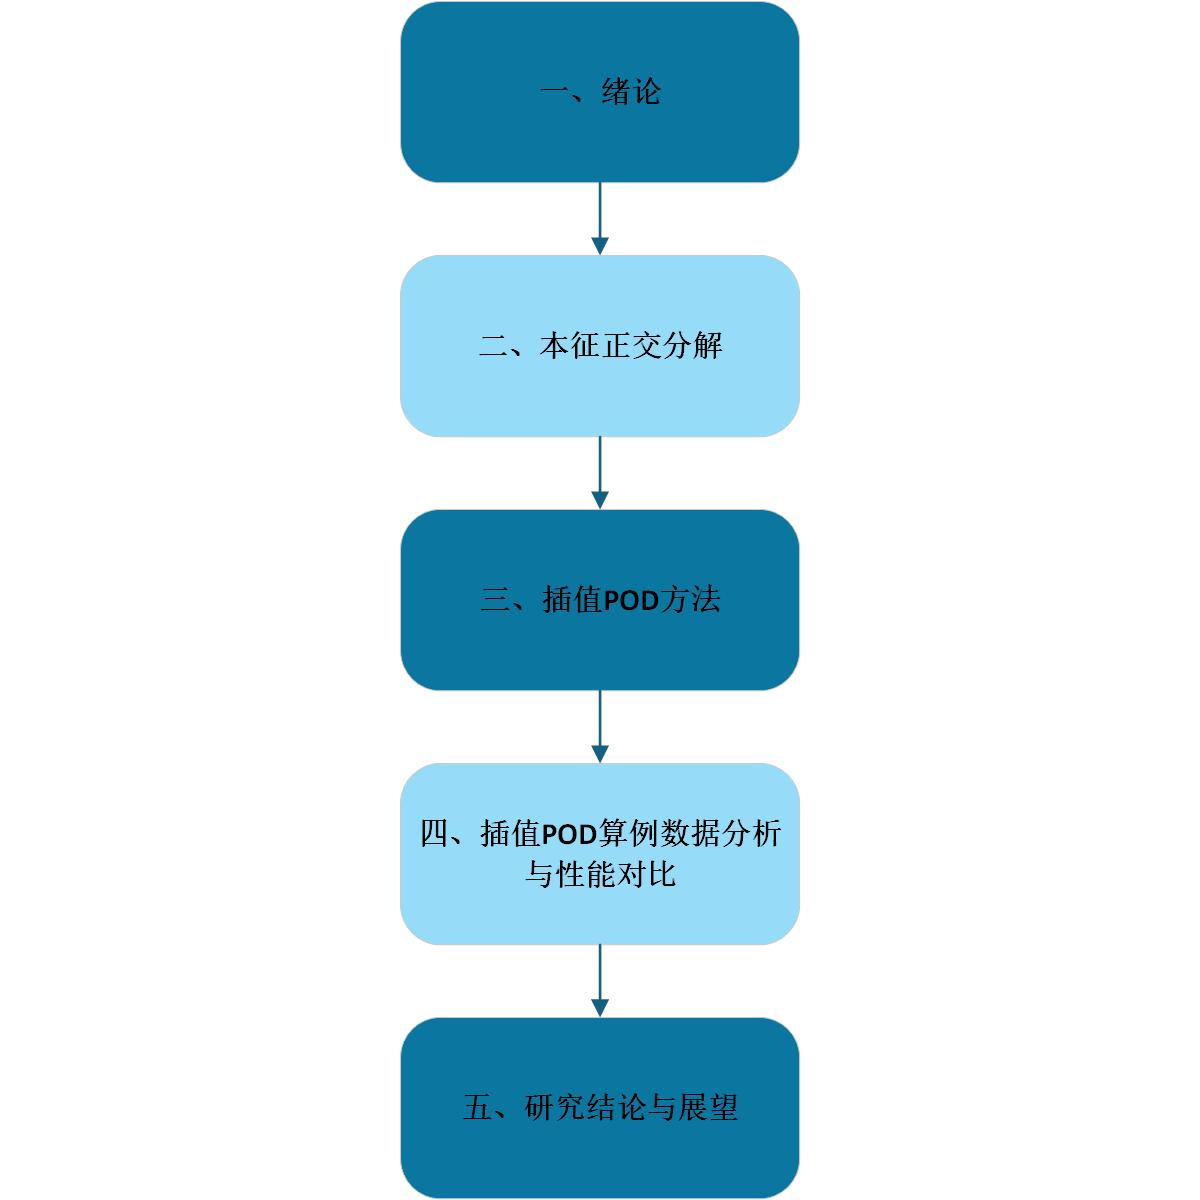
\includegraphics[width=1.0\linewidth]{论文结构图.jpg}
    \caption{论文组织结构图}
    \label{fig:enter-label}
\end{figure}
本章通过分析工程需求、梳理研究现状及明确技术路径,为后续 POD 理论推导、翼型模型建立及重构方法实现奠定基础。